\documentclass[tikz,border=10pt]{standalone}
% No extra TikZ libraries needed
\begin{document}
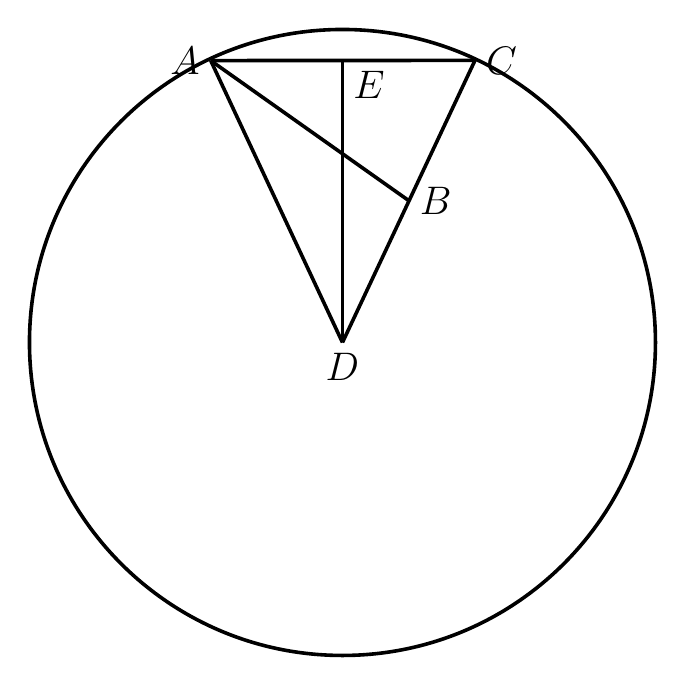
\begin{tikzpicture}[line join=round, line width=1.3pt]
  % Coordinates: origin at D, s = 0.016842 cm/px, y flipped
  \coordinate (D) at (0,0);
  \coordinate (A) at (-1.673,3.580);  % (176.7,62.1)
  \coordinate (C) at (1.683,3.582);   % (375.9,62.0)
  \coordinate (E) at (0,3.582);       % midpoint of AC
  \coordinate (B) at (0.844,1.800);   % (326.1,167.8), on CD

  % Circle centred at D, radius 236 px = 3.975 cm
  \draw (D) circle[radius=3.975];

  % Chord AC and the other segments
  \draw (A) -- (C);
  \draw (A) -- (B);
  \draw (C) -- (D);   % passes through B
  \draw (A) -- (D);
  \draw (E) -- (D);

  % Labels (no right-angle marks, no F label)
  \node[left,        font=\fontsize{13.5}{16.2}\selectfont] at (A) {$A$};
  \node[right,       font=\fontsize{13.5}{16.2}\selectfont] at (C) {$C$};
  \node[right,       font=\fontsize{13.5}{16.2}\selectfont] at (B) {$B$};
  \node[below,       font=\fontsize{13.5}{16.2}\selectfont] at (D) {$D$};
  % E sits just below the chord, right of the vertical line
  \node[below right, font=\fontsize{13.5}{16.2}\selectfont] at (E) {$E$};
\end{tikzpicture}
\end{document}